\section{Results and Discussion}

\section{Standard Evolutionary Experiments}

\begin{figure}%[!htbp]

\begin{center}
\setlength\tabcolsep{1.5pt} % default value: 6pt
\medmuskip=-2mu
\thinmuskip=-2mu
\thickmuskip=-2mu
\nulldelimiterspace=-1pt
\scriptspace=0pt
\begin{tabular}{ | c || c c c | c c c | }
  \multicolumn{1}{c}{} & \multicolumn{3}{c}{Competitors} & \multicolumn{3}{c}{Mean Dominant ($\pm S.D.$)} \\
 \cline{2-7}
  \multicolumn{1}{c|}{} & \tiny{$P_{1} = 1.0$} & \tiny{$P_{2} = P_{1}$} & \tiny{$P_{2} > P_{1}$} & \tiny{$P_{1} = 1.0$} & \tiny{$1.0 > P_{1} > P_{2}$} & \tiny{$P_{2} \geq P_{1}$}  \\
 \hline
 $n$ & 1 & 1 & 1 & 9 & 7 & 34  \\
 \hhline{|=||===|===|}
 $A_1$ & 0.00 & 1.00 & 1.00 & $0.23 \pm 0.35$ & $0.50 \pm 0.47$ & $0.57 \pm 0.46$ \\
 $A_2$ & 1.00 & 0.91 & 1.00 & $1.00 \pm  0.00$ & $1.00 \pm 0.00$ & $1.00 \pm 0.00$ \\
 \hline
 $P_{c}$ & 0.85 & 0.00 & 0.00 & $0.00 \pm 0.00$ & $0.00 \pm 0.00$ & $0.03 \pm 0.05$ \\
 $P_1$ & 0.07 & 1.00 & 0.00 & $1.00 \pm 0.00$ & $0.60 \pm 0.07$ & $0.28 \pm 0.16$ \\
 $P_2$ & 0.08 & 0.00 & 1.00 & $0.00 \pm 0.00$ & $0.40 \pm 007$ & $0.69 \pm 0.14$ \\
 \hline
 $C_1$ & 21.8 & 7.2 & 9.9 & $3.90 \pm 0.60$ & $3.38 \pm 0.33$ & $3.03 \pm 0.69$ \\
 $C_2$ & 101.2 & 274.2 & 238.2 & $230.6 \pm 71.1$ & $192.7 \pm 45.3$ & $271.6 \pm 73.6 $ \\
 \hline
 $E_{c}$ & 0.21 & 0.00 & 0.00 & $0.29 \pm 0.37$ & $0.44 \pm 0.59$ & $0.21 \pm 0.75$ \\
 $E_1$ & 1.21 & 30.1 & 0.00 & $47.2 \pm 21.7$ & $21.3 \pm 12.0$ & $4.62 \pm 7.05$ \\
 $E_2$ & 2.49 & 54.1 & 38.8 & $231.2 \pm 94.3$ & $283.1 \pm 57.0$ & $325.4 \pm 68.9$ \\
 \hline
 $M_{c}$ & 0.53 & 0.30 & 0.90 & $0.33 \pm 0.41$ & $0.74 \pm 0.31$ & $0.67 \pm 0.35$ \\
 $M_1$ & 1.00 & 0.00 & 1.00 & $0.52 \pm 0.41$ & $0.65 \pm 0.46$ & $0.68 \pm 0.38$ \\
 $M_2$ & 0.00 & 1.00 & 0.24 & $0.45 \pm 0.39$ & $0.52 \pm 0.37$ & $0.50 \pm 0.42$ \\
 \hline
 $S_1$ & 0.56 & 1.00 & 0.68 & $0.65 \pm 0.38$ & $0.55 \pm 0.40$ & $0.47 \pm 0.42$ \\
 $S_2$ & 1.00 & 0.84 & 0.71 & $0.51 \pm 0.43$ & $0.35 \pm 0.39$ & $0.45 \pm 0.39$ \\
 \hline
\end{tabular}
\end{center}
\caption{
Enumerations for genotypes used as seeds for competition experiments (left) and enumerations for mean values of the most abundant genotype at the end of evolutionary runs (right), both sorted by resource-caching strategy.
}
\label{fig:genotypes}
\end{figure}


\begin{figure}[t]
\begin{center}
\begin{subfigure}[b]{0.82\columnwidth}
  \includegraphics[width=\columnwidth,trim={2.5cm 0.5cm 2.5cm 1cm},clip]{img/ChannelMap_1022_update19500000}
  \caption{Mean $P_0 = 0.77$, $P_1 = 0.089$, $P_2 = 0.14$; generation 20,475}
  \label{fig:ChannelMap_1022}
\end{subfigure}

\begin{subfigure}[b]{0.82\columnwidth}
  \includegraphics[width=\columnwidth,trim={2.5cm 0.5cm 2.5cm 1cm},clip]{img/ChannelMap_1041_update19500000}
  \caption{Mean $P_1 = 1.0$; generation 23,971}
  \label{fig:ChannelMap_1041}
\end{subfigure}

\begin{subfigure}[b]{0.82\columnwidth}
  \includegraphics[width=\columnwidth,trim={2.5cm 0.5cm 2.5cm 1cm},clip]{img/ChannelMap_1008_update19500000}
  \caption{Mean $P_2 = 1.0$; generation 25,841}
  \label{fig:ChannelMap_1008}
\end{subfigure}

\caption{
State of same-channel zero- and one-level signaling networks after $19.5$ million updates of evolution with different population mean $P_0$, $P_1$, and $P_2$.
Zero-level channels coded by HSV value are separated by white borders and one-level channels coded by HSV hue are separated by black borders.
}
\label{fig:outcome_grids}
\end{center}
\end{figure}


\begin{figure}[t]
\begin{center}
\begin{subfigure}[b]{0.5\columnwidth}
  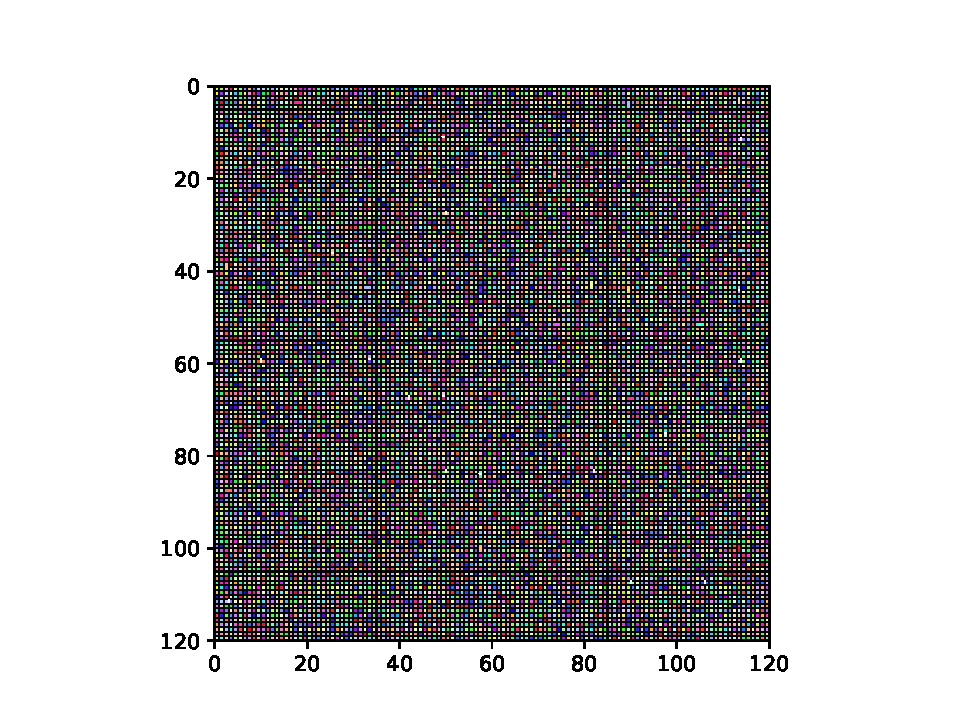
\includegraphics[width=\columnwidth,trim={2.5cm 0.5cm 2.5cm 1cm},clip]{img/ChannelMap_1011_update0}
  \caption{Update 0 (Generation 0)}
  \label{fig:ChannelMap_1011_update0}
\end{subfigure}%
\begin{subfigure}[b]{0.5\columnwidth}
  \includegraphics[width=\columnwidth,trim={2.5cm 0.5cm 2.5cm 1cm},clip]{img/ChannelMap_1011_update1000000}
  \caption{Update 1 million (Generation 927)}
  \label{fig:ChannelMap_1011_update1000000}
\end{subfigure}
\begin{subfigure}[b]{0.5\columnwidth}
  \includegraphics[width=\columnwidth,trim={2.5cm 0.5cm 2.5cm 1cm},clip]{img/ChannelMap_1011_update2000000}
  \caption{Update 2 million (Generation 1917)}
  \label{fig:ChannelMap_1011_update2000000}
\end{subfigure}%
\begin{subfigure}[b]{0.5\columnwidth}
  \includegraphics[width=\columnwidth,trim={2.5cm 0.5cm 2.5cm 1cm},clip]{img/ChannelMap_1011_update4000000}
  \caption{Update 4 million (Generation 4053)}
  \label{fig:ChannelMap_1011_update4000000}
\end{subfigure}
\begin{subfigure}[b]{0.5\columnwidth}
  \includegraphics[width=\columnwidth,trim={2.5cm 0.5cm 2.5cm 1cm},clip]{img/ChannelMap_1011_update5000000}
  \caption{Update 5 million (Generation 5173)}
  \label{fig:ChannelMap_1011_update5000000}
\end{subfigure}%
\begin{subfigure}[b]{0.5\columnwidth}
  \includegraphics[width=\columnwidth,trim={2.5cm 0.5cm 2.5cm 1cm},clip]{img/ChannelMap_1011_update7000000}
  \caption{Update 7 million (Generation 7312)}
  \label{fig:ChannelMap_1011_update7000000}
\end{subfigure}
\caption{
Progression of of same-channel level-zero and level-one signaling networks states in an evolutionary run where population mean $P_1 > P_{self}, P_0$ evolved.
Level-zero channels coded by HSV value are separated by white borders and level-one channels coded by HSV hue are separated by black borders.
}
\label{fig:grid_progression}
\end{center}
\end{figure}


A spectrum of resource allocation strategies were observed at the conclusion of different runs of our evolutionary simulation (mean generation 37,168; $s=4,684$).
We interpret these outcomes as ranging between first-level and second-level individuality.
The criteria used to discern these outcomes are described below.
Figure \ref{fig:outcome_grids} shows the level-one and level-two signaling networks at the end of runs where first-, split-, and second-level resource allocation evolved, respectively.
First-level individuals form somewhat irregular level-two amalgamations of diverse level-one networks.
Second-level individuals form highly regular diamond-shaped level-two signaling networks.
Split-allocation individuals exhibit a level-two phenotype of intermediate regularity.
Figure \ref{fig:grid_progression} shows a time series of signaling network snapshots in an evolutionary run where second-level individuality evolved.

Figure \ref{fig:genotypes} describes predominant genotypes observed at the end of our evolutionary simulations.
All evolved genotypes had $A_2$ fixed at $1.0$.
So, reproduction over cells sharing the same level-two channel was universally avoided;
genotypes evolved so that cells declined to reproduce when they were located at the interior of level-two same-channel signaling networks.

However, a variety of resource-caching strategies evolved.
Most-abundant genotypes at the end of evolutionary runs included strategies where resource was primarily cached in an organism's individual stockpile (i.e., $P_{c} > P_1, P_2$), strategies where resource was primarily cached in an organism's level-one signaling network's pool (i.e., $P_1 > P_{c}, P_2$), and strategies where resource was primarily cached in an organism's level-two signaling network's pool (i.e., $P_2 > P_{c}, P_1$).
Among 50 trials, pure first-level allocation dominated at the end of nine replicates, primarily level-one split resource-sharing dominated in seven replicates, and primarily level-two split resource sharing dominated in 34 replicates.
We suspect that a trade-off between growth rate and long-term stability contributed to our observation of split resource sharing strategies.
Cell- and level-one resource caching might function something like saving for a rainy day.
Because reproduction over level-two channel-mates was universally avoided, cells and level-one same-channel networks situated at the interior of a larger level-two same-channel network do not expend their resource pools unless the larger level-one same-channel network is damaged, exposing them to directly-adjacent cells of a different level-one channel.
Thus, resource accumulates in cells and level-one pools until the level-one same-channel network comes under stress.
Split allocation might also represent hedging against defection of a second-level channel-mate by via mutation.

We selection for apoptosis
Excluding replicates where exclusive first-level resource caching dominated, standard evolutionary runs at update 20 million, mean population mean $M_{c}$ was $0.67$, standard deviation 0.33, $n=42$.
This is significantly greater than the value $M_{c} = 0.5$ we would expect in the absence of a selective pressure for an apoptosis response to mutation ($p < 0.05$, test TODO).

\begin{figure}[t]
\begin{center}

\begin{subfigure}[b]{\columnwidth}
  \includegraphics[width=\columnwidth]{img/champion_res_pool1_vs_champion_damage_suicide0}
  \label{fig:champion_res_pool1_vs_champion_damage_suicide0}
\end{subfigure}

\begin{subfigure}[b]{\columnwidth}
  \includegraphics[width=\columnwidth]{img/champion_res_pool2_vs_champion_damage_suicide0}
  \label{fig:champion_res_pool2_vs_champion_damage_suicide0}
\end{subfigure}

\caption{
TODO
}
\label{fig:damage_suicide}
\end{center}
\end{figure}


To assess whether higher-level individuals were more likely to employ apoptosis to mitigate somatic mutation, we examined the relationship between first- and second-level resource pooling and cellular apoptosis at the conclusion of our 33 replicate evolutionary trials.
We observed a significant negative correlation between dominant genotype $P_1$ and $M_{c}$ ($p < 0.05$; bootstrap test; Figure \ref{fig:champion_res_pool1_vs_champion_damage_suicide0}) and a significant positive correlation between dominant genotype $P_2$ and $M_{c}$ ($p < 0.05$; bootstrap test; Figure \ref{fig:champion_res_pool2_vs_champion_damage_suicide0}).
This result suggests that second-level individuals, in particular, relied on apoptosis to mitigate somatic mutation.


To assess whether higher-level individuals provided larger resource endowments to their propagules (offspring sharing neither the level-one nor the level-two channel ID with the parent), we examined the relationship between first and second-level resource pooling and dominant genotype second-level propagule endowment at the conclusion of our 50 replicate evolutionary trials.
We observed a significant negative correlation between dominant genotype $P_1$ and $E_2$ ($p < 0.05$; bootstrap test) and a significant positive correlation between dominant genotype $P_2$ and $E_2$ ($p <  0.005$; bootstrap test).
Second-level individuals might provide larger endowments to propagules simply due to a greater capacity to collect resource or perhaps because of stronger selection for well-endowed offspring when competing against other second-level individuals.

We also observed a significant positive correlation between first-level resource sharing and first-level endowment ($p < 0.0001$; bootstrap test) and a significant negative correlation between second-level resource sharing and first-level endowment ($p < 0.0001$; bootstrap test).

\subsection{Competition Experiments}

\begin{figure*}%[!htbp]
\begin{center}


\begin{subfigure}[b]{0.9\columnwidth}
  \includegraphics[width=\columnwidth,trim={2.5cm 0.5cm 2.5cm 1cm},clip]{img/ChannelMap_1030_update0}
  \caption{Update 0; cell gen. 0}
  \label{fig:ChannelMap_1030_update0}
\end{subfigure}%
\begin{subfigure}[b]{0.9\columnwidth}
  \includegraphics[width=\columnwidth,trim={2.5cm 0.5cm 2.5cm 1cm},clip]{img/ChannelMap_1030_update5552}
  \caption{Update 5552; cell gen. 4}
  \label{fig:ChannelMap_1030_update55520}
\end{subfigure}

\begin{subfigure}[b]{0.9\columnwidth}
  \includegraphics[width=\columnwidth,trim={2.5cm 0.5cm 2.5cm 1cm},clip]{img/ChannelMap_1030_update11104}
  \caption{Update 1104; cell gen. 9}
  \label{fig:ChannelMap_1030_update277600}
\end{subfigure}%
\begin{subfigure}[b]{0.9\columnwidth}
  \includegraphics[width=\columnwidth,trim={2.5cm 0.5cm 2.5cm 1cm},clip]{img/ChannelMap_1030_update22208}
  \caption{Update 22208; cell gen. 32}
  \label{fig:ChannelMap_1030_update22208}
\end{subfigure}

\begin{subfigure}[b]{0.9\columnwidth}
  \includegraphics[width=\columnwidth,trim={2.5cm 0.5cm 2.5cm 1cm},clip]{img/ChannelMap_1030_update55520}
  \caption{Update 55520; cell gen. 107}
  \label{fig:ChannelMap_1030_update1000000}
\end{subfigure}%
\begin{subfigure}[b]{0.9\columnwidth}
  \includegraphics[width=\columnwidth,trim={2.5cm 0.5cm 2.5cm 1cm},clip]{img/ChannelMap_1030_update1500000}
  \caption{Update 1500000; cell gen. 3511}
  \label{fig:ChannelMap_1030_update1500000}
\end{subfigure}
\caption{
Progression of of same-channel level-one and level-two signaling networks states in an evolutionary run where level-two resource sharing evolved.
Level-one channels are coded by color saturation and level-two channels are coded by color hue.
A single cell-like organism occupies each grid tile except for black tiles, which are empty.
}
\label{fig:eco_progression}
\end{center}
\end{figure*}


\begin{figure}%[!htbp]
\begin{center}

\includegraphics[width=\columnwidth,trim={2.5cm 0.5cm 2.5cm 1cm},clip]{img/ChannelMap_1018_update3000000}

\caption{
End state (update 3000000, cell gen. 6916) of same-channel signaling networks evolved under the control treatment.
Level-one channels are coded by color saturation and level-two channels are coded by color hue.
A single cell-like organism occupies each grid tile except for black tiles, which are empty.
Level-one same-channel groups appear as uniformly-colored clumps, bounded by a white border.
Level-two same-channel groups appear as same-hue amalgamations of level-one groups, bounded by a black border.
}
\label{fig:outcome_control}
\end{center}
\end{figure}


Next, we wanted to compare cell-, first-, and second-level individuals to determine which genotype was the most fit in the DISHTINY platform environment.
We ran competition experiments between the the dominant genotypes from the run with greatest mean $P_{c}$, the run with greatest mean $P_1$, and the run with greatest mean $P_2$.
The a mean of $90.2 \%$ of the , standard deviation $3.8 \%$.
%In 22 out of 191 trials performed fixation was reached by update 1.5 million.
TODO replace with info on dominance
The second-level resource caching strategy was most abundant at update 1.5 million of all 50 trials.
These results show that in the absence of mutation, second-level individuals tend to exhibit greater fitness than evenly-split-allocation and first-level individuals ($p < 0.0001$; two-tailed exact test).

Figure \ref{fig:eco_progression} shows a time series of signaling network snapshots in an competition experiment run.
Colonies of each genotype can be seen to grow from each seed and then clash, yielding

\begin{figure}[!htbp]
\begin{center}

\begin{subfigure}[b]{0.5\columnwidth}
  \includegraphics[width=\columnwidth]{img/mean_res_pool1_vs_net_reproduction}
  \caption{
  Correlation plot of population mean $P_0$ and population net reproduction rate.
  }
  \label{fig:mean_res_pool1_vs_net_reproduction}
\end{subfigure}%
\begin{subfigure}[b]{0.5\columnwidth}
  \includegraphics[width=\columnwidth]{img/mean_res_pool2_vs_net_reproduction}
  \caption{
  Correlation plot of population mean $P_1$ and population net reproduction rate.
  }
  \label{fig:mean_res_pool2_vs_net_reproduction}
\end{subfigure}
\caption{
Mean resource caching strategies and net reproduction rate across populations.
A bootstrapped 95\% confidence interval for the fit is shaded.
}
\label{fig:net_reproduction}
\end{center}
\end{figure}


In competition experiments, however, higher-level individuals likely benefited from elimination of somatic mutation.
To assess the relative fitness of first- and second-level individuals without mutation disabled, we examined the relationship between first- and second-level resource pooling and the rate of cellular reproduction at the end of each of the 50 replicate evolutionary trials performed.
We observed a significant negative correlation between mean $P_1$ and cellular reproduction rate ($p < 0.0001$; bootstrap test; Figure \ref{fig:mean_res_pool1_vs_net_reproduction}) and a significant positive correlation between mean $P_2$ and cellular reproduction rate ($p < 0.0001$; bootstrap test; Figure \ref{fig:mean_res_pool2_vs_net_reproduction}).
This result suggests that second-level individuals tend to collect resource more effectively than evenly-split-allocation and first-level individuals.

\subsection{Control Evolutionary Experiments}

larger same-channel networks

less apoptosis
selected AGAINST
